\documentclass[a4paper,11pt,fleqn]{article}%fleqn pour aligner les equations à gauche
\usepackage{../../Styles/Cours}

\newcommand{\chnum}{Chapitre 1}
\newcommand{\chtitle}{Règles et matériel du laboratoire}
\newcommand{\dtype}{TP}

\begin{document}
\maketitle

\section{Règles en salle de TP}
La sécurité est l’un des enjeux majeurs en cours de Sciences Physiques et Chimiques. Pour cela chacun doit respecter au sein de la classe des consignes de sécurités simples :
\begin{itemize}
	\item Porter une blouse en coton, un pantalon et des chaussures fermées pour protéger votre peau.
	\item Les cheveux longs doivent être attachés.
	\item Mettre des lunettes et des gants pour manipuler les produits dangereux.
	\item Manipuler debout près de la paillasse.
	\item Bien ranger les sacs au fond de la salle ou sous la paillasse, ne prendre que la paillasse que le strict nécessaire.
	\item Ne pas circuler dans la classe en portant des produits dangereux.
	\item Ne prélever aucun solide avec les doigts, utiliser une spatule.
	\item Toujours reboucher un flacon après usage.
	\item Ne jamais essayer de reconnaître un produit à son odeur.
	\item Ne jamais prélever le produit dans le flacon du laboratoire, le verser d’abord dans un bécher.
	\item En fin de manipulation, demander au professeur si les solutions peuvent être jetées à l’évier ou si elles doivent être versées dans les bacs de récupération.
	\item A la fin de la séance, nettoyer et ranger votre matériel. Lavez-vous les mains.
\end{itemize}

\section{Signalétique}

Les produits chimiques peuvent être dangereux et connaître la signification des pictogrammes de sécurité pour travailler en toute sécurité.
\textit{Associer les termes suivants aux différents pictogrammes : Inflammable, Dangereux, Sous pression, Explosif, Mortel, Dangereux pour l’environnement, Corrosif, Cancérigène, Comburant (fait brûler).}\\
\begin{center}
	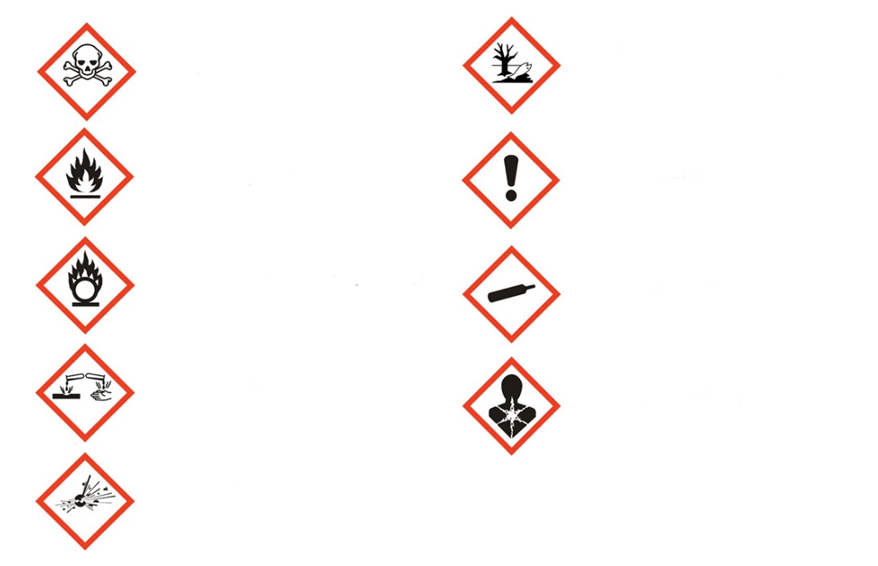
\includegraphics[scale=.5]{Ressources/2GT_TP0_Fig1.png}
\end{center}

\section{Matériel}
En chimie, vous devrez connaître les noms des principaux éléments de verrerie et leurs schéma respectifs.
\renewcommand{\arraystretch}{4}
\begin{table}[h!]
	\begin{tabular}{|>{\centering}m{3cm}|>{\centering}m{5.5cm}||>{\centering}m{3cm}|>{\centering\arraybackslash}m{5.5cm}|}
	\hline
	\textbf{Nom} & \textbf{Schéma} & \textbf{Nom} & \textbf{Schéma}\\ \hline
	Cristallisoir & & Ballon à fond plat & \\ \hline
	Bécher & & Ballon à fond rond & \\ \hline
	Erlenmeyer & & Verre à pied & \\ \hline
	Flacon & & Tube à essai & \\ \hline
	Capsule de pesée / Coupelle & & Pipette & \\ \hline
	\end{tabular}
\end{table}
\vspace{1em}

\begin{table}[h!]
\begin{tabular}{|>{\centering}m{2.3cm}|>{\centering}m{2.2cm}|>{\centering}m{2.3cm}|>{\centering}m{2.3cm}|>{\centering}m{2.2cm}|>{\centering}m{2.2cm}|>{\centering\arraybackslash}m{2.2cm}|}
	\hline
	&&&&&&\rule[5cm]{0cm}{0cm}\\ \hline
	Pipette graduée & Pipette Jaugée & Éprouvette graduée & Fiole jaugée & Entonnoir & Ampoule à décanter & Réfrigérant \\ \hline 
\end{tabular}
\end{table}
\end{document}
